% Final PIBIC-ITA report, English version
% Template based on the official ITA instructions
\documentclass[12pt,a4paper]{article}

% Required packages
\usepackage{iftex}
\ifPDFTeX
\usepackage[utf8]{inputenc}
\fi
\usepackage[british]{babel}
\babelhyphenation{ad-vances}
\babelhyphenation{laurent varoquaux}
\babelhyphenation{accelerator}
\babelhyphenation{xgboost resgatedgcn marinho}
\babelhyphenation{cor-re-spond cor-re-sponds cor-re-spond-ence log-arith-mic smaller}
\ifPDFTeX
\usepackage[T1]{fontenc}
\fi
\usepackage{geometry}
\usepackage{setspace}
\usepackage{graphicx}
\usepackage{float}
\usepackage{caption}
\usepackage{subcaption}
\captionsetup[sub]{font=normalsize}
\usepackage{tabularx}
\usepackage{booktabs}
\usepackage{multirow}
\usepackage{array}
\usepackage{amsmath}
\usepackage{amsfonts}
\usepackage{amssymb}
\usepackage{fancyhdr}
\usepackage{titlesec}
\usepackage{tocloft}
\usepackage{url}
\usepackage{siunitx}
\usepackage{tikz}
\usepackage[round]{natbib}
\usepackage{hyperref}

% Page layout
\geometry{
    top=2cm,
    bottom=2cm,
    left=2cm,
    right=2cm
}

% Font: Arial (Helvetica) 12
\ifPDFTeX
\usepackage{newtxtext,newtxmath}
\else
\usepackage[no-math]{fontspec}
\setsansfont{texgyreheros}[Extension=.otf, UprightFont=*-regular, BoldFont=*-bold, ItalicFont=*-italic, BoldItalicFont=*-bolditalic]
\renewcommand{\rmdefault}{minntx}
\usepackage{newtxmath}
\setmainfont{texgyreheros}[Extension=.otf, UprightFont=*-regular, BoldFont=*-bold, ItalicFont=*-italic, BoldItalicFont=*-bolditalic]
\fi
\renewcommand{\familydefault}{\sfdefault}

% Units with the decimal point and English list and range words
\sisetup{
    output-decimal-marker = {.},
    per-mode              = symbol,
    mode                  = match,
    reset-text-family     = false,
    list-final-separator  = {\ \text{and}\ },
    list-pair-separator   = {\ \text{and}\ },
    range-phrase          = {\ \text{to}\ }
}
\DeclareSIUnit{\pe}{p.e.}

% Line spacing 1.5
\onehalfspacing
\widowpenalty=10000

% hyperref configuration
\hypersetup{
    colorlinks=true,
    linkcolor=black,
    filecolor=magenta,
    urlcolor=blue,
    citecolor=black
}

% Bibliography: links in the text font, each DOI printed as a link to https://doi.org,
% and the list single-spaced with a ragged right margin, as abntex2cite sets it in the Portuguese version
\urlstyle{same}
\makeatletter
\DeclareRobustCommand*{\doi}{\begingroup\catcode`\_=12 \catcode`\%=12 \catcode`\#=12 \doi@link}
\newcommand*{\doi@link}[1]{\endgroup doi:~\href{https://doi.org/#1}{\nolinkurl{#1}}}
\renewcommand{\bibfont}{\setstretch{1}\setlength{\@rightskip}{0pt plus 2cm}}
\makeatother

% Section heading format
\titleformat{\section}{\normalfont\large\bfseries}{\thesection}{1em}{}
\titleformat{\subsection}{\normalfont\normalsize\bfseries}{\thesubsection}{1em}{}

% Header and footer
\pagestyle{fancy}
\fancyhf{}
\renewcommand{\headrulewidth}{0pt}
\cfoot{\thepage}

% Project variables
\newcommand{\tituloprojeto}{Performance Studies of the APE Photon~System}
\newcommand{\nomealuno}{Victor Elias Vicentin}
\newcommand{\emailaluno}{victor.vicentin.8856@ga.ita.br}
\newcommand{\telefonealuno}{}
\newcommand{\nomeorientador}{Prof.~Dr.~Franciole da Cunha Marinho}
\newcommand{\emailorientador}{franciole@ita.br}
\newcommand{\telefoneorientador}{}
\newcommand{\mesano}{October 2026}
\newcommand{\datacompleta}{14 October 2026}

\begin{document}
\frenchspacing

% ========== COVER ==========
% File: capa.tex
% Cover of the PIBIC-ITA report

\thispagestyle{empty}
% Logos side by side
\begin{center}
  \begin{minipage}{0.45\textwidth}
    \flushleft
    
\includegraphics[width=3cm]{logos/ita.png}
  \end{minipage}
  \hfill
  \begin{minipage}{0.45\textwidth}
    \flushright
    
\includegraphics[width=3cm]{logos/cnpq.jpg}
  \end{minipage}
    \rule{\textwidth}{0.4pt} % horizontal rule
\end{center}

\begin{center}

% Header with the titles at the top and a horizontal rule
\begin{center}
  {\large \textbf{AERONAUTICS INSTITUTE OF TECHNOLOGY}}\\[0.3cm]
  {\large \textbf{NATIONAL COUNCIL FOR SCIENTIFIC AND}}\\
  {\large \textbf{TECHNOLOGICAL DEVELOPMENT - CNPq}}\\[0.3cm]

\end{center}

\vspace{0.3cm}




\vspace{1.5cm}

{\Large \textbf{INSTITUTIONAL PROGRAMME OF SCIENTIFIC}}\\[0.2cm]
{\Large \textbf{INITIATION SCHOLARSHIPS - PIBIC}}

\vspace{0.3cm}

{\large \textbf{Coordination of the Scientific and Technological}}\\
{\large \textbf{Initiation Activities Programme of ITA}}

%\vspace{0.3cm}

%{\large \textbf{caic@ita.br}}

\vspace{2cm}

% Project title
{\LARGE \setstretch{1}\textbf{\tituloprojeto}\par}

\vspace{2cm}

% Student's name
{\Large \textbf{\nomealuno}}

\vspace{2cm}

% Report type
{\Large \textbf{FINAL ACTIVITY REPORT}}

\vspace{2cm}

% Supervisors
\begin{tabular}{@{}l@{}}
\textbf{Supervisor:} \nomeorientador \\
\end{tabular}

\vspace{2cm}

% Date
São José dos Campos, \datacompleta

\end{center}

% ========== SIGNATURE SHEET ==========
\newpage
% File: assinaturas.tex
% Signature sheet of the PIBIC-ITA report

\thispagestyle{empty}

% Logos side by side
\begin{center}
  \begin{minipage}{0.45\textwidth}
    \flushleft
    
\includegraphics[width=3cm]{logos/ita.png}
  \end{minipage}
  \hfill
  \begin{minipage}{0.45\textwidth}
    \flushright
    
\includegraphics[width=3cm]{logos/cnpq.jpg}
  \end{minipage}
    \rule{\textwidth}{0.4pt} % horizontal rule
\end{center}

\begin{center}

% Header with the titles at the top and a horizontal rule
\begin{center}
  {\large \textbf{AERONAUTICS INSTITUTE OF TECHNOLOGY}}\\[0.3cm]
  {\large \textbf{NATIONAL COUNCIL FOR SCIENTIFIC AND}}\\
  {\large \textbf{TECHNOLOGICAL DEVELOPMENT - CNPq}}\\[0.3cm]

\end{center}

\vspace{1cm}

{\large \textbf{Final Activity Report}}

\vspace{1cm}

{\Large \setstretch{1}\textbf{\tituloprojeto}\par}

\vspace{2cm}

% Signature tables
\begin{tabular}{|p{5cm}|p{10cm}|}
\hline
\textbf{Student's name} & \nomealuno \\
\hline
\textbf{Student's signature} & \\[0.9cm]
\hline
\textbf{Student's telephone} & \telefonealuno \\
\hline
\textbf{Student's email} & \emailaluno \\
\hline
\end{tabular}

\vspace{1cm}

\begin{tabular}{|p{5cm}|p{10cm}|}
\hline
\textbf{Supervisor's name} & \nomeorientador \\
\hline
\textbf{Supervisor's signature} & \\[0.9cm]
\hline
\textbf{Supervisor's telephone} & \telefoneorientador \\
\hline
\textbf{Supervisor's email} & \emailorientador \\
\hline
\end{tabular}

\vspace{1cm}

%%%COMMENT OUT IF THERE IS NO CO-SUPERVISOR
%\begin{tabular}{|p{5cm}|p{10cm}|}
%\hline
%\textbf{Co-supervisor's name} & \nomecoorientador \\
%\hline
%\textbf{Co-supervisor's signature} & \\[0.9cm]
%\hline
%\textbf{Co-supervisor's telephone} & \telefonecoorientador \\
%\hline
%\textbf{Co-supervisor's email} & \emailcoorientador \\
%\hline
%\end{tabular}

\end{center}

% ========== APPROVAL FORM ==========
\newpage
% File: aprovacao.tex
% Report approval form filled in by the supervisor

\thispagestyle{empty}

% Logos side by side
\begin{center}
  \begin{minipage}{0.45\textwidth}
    \flushleft
    
\includegraphics[width=3cm]{logos/ita.png}
  \end{minipage}
  \hfill
  \begin{minipage}{0.45\textwidth}
    \flushright
    
\includegraphics[width=3cm]{logos/cnpq.jpg}
  \end{minipage}
    \rule{\textwidth}{0.4pt} % horizontal rule
\end{center}

% Header with the titles at the top and a horizontal rule
\begin{center}
  {\large \textbf{AERONAUTICS INSTITUTE OF TECHNOLOGY}}\\[0.3cm]
  {\large \textbf{NATIONAL COUNCIL FOR SCIENTIFIC AND}}\\
  {\large \textbf{TECHNOLOGICAL DEVELOPMENT - CNPq}}\\[0.3cm]

\end{center}

\vspace{1cm}

% Table with check boxes
\begin{tabular}{|p{6cm}|p{4cm}|p{4cm}|}
  \hline
  \textbf{Report:} & Partial $\square$ & Final $\boxtimes$ \\
  \hline
\end{tabular}

\vspace{0.3cm} % reduced from 1cm to 0.3cm

% Block 1 - Assessment of the aspects
\begin{center}
\fbox{
\begin{minipage}{0.9\textwidth}\raggedright
\textbf{1- I CONSIDER THE REPORT APPROVED ON THE BASIS OF THE~FOLLOWING \mbox{ASPECTS}}

\vspace{0.5cm} % small space after the heading

 Space to be filled in
\vspace{4cm}
\end{minipage}
}
\end{center}

\vspace{0.3cm}

% Block 2 - Assessment of the performance
\begin{center}
\fbox{
\begin{minipage}{0.9\textwidth}\raggedright
\textbf{2- THE SUPERVISOR'S ASSESSMENT OF THE SCHOLARSHIP HOLDER'S PERFORMANCE IN THE SCIENTIFIC INITIATION WORK}

\vspace{0.5cm}

 Space to be filled in
\vspace{4cm}
\end{minipage}
}
\end{center}

\vspace{1cm} % space before the signature

São José dos Campos, \datacompleta

\vspace{0.5cm}

\textbf{Supervisor's signature:} \underline{\hspace{6cm}}


% ========== CONTENTS ==========
\newpage
\tableofcontents
\newpage

% ========== SUMMARY OF THE INITIAL PLAN ==========
\phantomsection
\section*{Summary of the Initial Plan}
\addcontentsline{toc}{section}{Summary of the Initial Plan}

\label{sec:resumo_plano}

The project, which ran from 1 September 2025 to 31 August 2026, continued the previous stage. In that stage, a dense neural network of \num{8195} parameters estimated the interaction vertex of \qty{10}{\MeV} deposits in the third far detector module (FD3) of the DUNE experiment (Deep Underground Neutrino Experiment) from \num{60} descriptors of the scintillation light \citep{vicentin2024study}.

The objective was to use machine learning to estimate the three-dimensional position of energy deposits of the order of MeV from the light recorded by a photon detection system of the APEX type (Aluminum Profiles with Embedded X-ARAPUCA), as a measure of the performance of that system. The plan envisaged measuring the spatial resolution in each coordinate and comparing it with that of the analytic estimators of the APEX study \citep{marinho2025apex}. The reconstruction would also be extended to other deposited energies and to other sensor geometries, as the conclusion of the previous stage proposed.

The methodology started from the simulation used in that stage, with the photon counts rescaled from \qty{100}{\MeV} to \qty{10}{\MeV} and binomial detection with an efficiency of \qty{2}{\percent}. The plan included a hyperparameter search, an evaluation on events held out for testing in terms of the mean absolute error (MAE), the root-mean-square error (RMSE) and the coefficient of determination ($R^2$) along each axis, and a study as a function of energy and efficiency. The expected outcome was a per-coordinate resolution better than that of the previous stage, whose test MAE ranged from \num{12.03} to \qty{18.18}{\cm} per axis \citep{vicentin2024study}, and better than that of the analytic estimators, with a model lightweight enough for use in real-time data acquisition. The results would be presented at the 2026 Scientific Initiation Meeting of the Aeronautics Institute of Technology (ENCITA) and in this report.


\newpage

% ========== SUMMARY OF THE ACTIVITIES CARRIED OUT ==========
\phantomsection
\section*{Summary of the Activities Carried Out}
\addcontentsline{toc}{section}{Summary of the Activities Carried Out}

\label{sec:resumo_atividades}

The work used the simulated events of the previous stage, whose files date from October 2025: \qty{100}{\MeV} deposits, rescaled to \qty{10}{\MeV}, in one octant of the third far detector module (FD3) of DUNE (Deep Underground Neutrino Experiment), read out by \num{6912} channels. In December 2025, a prototype graph neural network (GNN) was tested, followed, in February and March 2026, by the GATv2 and GPS encoders, with a hierarchical regression head. In June, the code was rebuilt as an installable package; the work corrected two geometry defects and three hot channels, mirrored the training events into the other octants and restricted the graphs to the lit channels, with \num{17} features per node and \num{23} per edge. In July, a simple gradient-boosting model outperformed the GNN of the time, and the XGBoost and LightGBM boosters were added as reference models.

On 4 August 2026, the boosters were tuned, and a first comparison trained \num{11} of the \num{14} encoders on a quarter of the training events. A diagnosis of the gap to the boosters led to the use of the \num{7490} training events and \num{33} event-level scalars, which summarise the event's light. In the final comparison of 8 August, the training of \num{11} matched-capacity encoders, with a maximum deviation of \qty{1.6}{\percent} from \num{1843395} parameters, totalled \qty{11.42}{\hour}.

In this report, without retraining, the boosters, tuned and trained on light with data augmentation, were re-evaluated on the same light as the encoders, and the confidence intervals and the light barycentre were computed, all on the same test events. The outputs are a paper with the results for the 2026 Scientific Initiation Meeting of the Aeronautics Institute of Technology (ENCITA), project slides and a repository of \num{155} commits and \num{172} Python files, with \num{18025} lines and \num{130} test functions.

On the \num{937} test events, the four encoders with the lowest error (two variants of GATv2 and two of GPS), indistinguishable from one another, have a mean three-dimensional error (mean distance from the predicted to the true vertex) of \num{25.95} to \qty{26.27}{\cm} and a root-mean-square error of the three axes together (combined RMSE) of \num{18.55} to \qty{18.80}{\cm}. XGBoost, on the same light, has a combined RMSE of \qty{20.95}{\cm}, but errs less on the brightest events. The network of the previous stage has \qty{20.86}{\cm}, a value computed from the published per-axis RMSE values, which come from a different partition \citep{vicentin2024study}. APEX (Aluminum Profiles with Embedded X-ARAPUCA), from a different simulation \citep{marinho2025apex}, has a combined width (root mean square of the resolution widths of the three axes, read from a plot) of \qty{38.0}{\cm} at the mean light per test event with its average light yield, \qty{31.8}{\cm} with the minimum and \qty{25.9}{\cm} at equal energy. In $z$, the long axis, against \num{20.15} to \qty{20.46}{\cm} for the four encoders, APEX has \qty{24.8}{\cm} with the average yield, above the confidence interval of each of them, and \qty{19.4}{\cm} with the minimum, within it; only at equal energy, where it detects \num{3.4} times as much light, is it better (\qty{13.7}{\cm}).


\newpage

% ========== PROBLEM DESCRIPTION ==========
\section{Problem Description}

\label{sec:problema}

\subsection{DUNE, FD3 and scintillation light}
\label{sec:detector}

DUNE (Deep Underground Neutrino Experiment) will study neutrino oscillation with a beam from Fermilab and a far detector \qty{1300}{\km} away; its goals include CP violation (charge conjugation and parity), the mass ordering, supernova neutrinos and proton decay \citep{abi2020volume}. According to \citet{abud2024dunephase}, the far detector uses liquid argon time projection chambers (LArTPCs); Phase~II adds the third module (FD3), a vertical drift module like the second (FD2); the photon detection system of FD3 will be defined by the APEX programme (Aluminum Profiles with Embedded X-ARAPUCA).

Charged particles ionise and excite the argon: the electrons drift to the readout planes, which give the coordinates perpendicular to the drift, and the scintillation (about \num{24000} photons per MeV at \qty{500}{\V\per\cm}, near \qty{127}{\nm}) marks the time $t_0$ of the interaction, on which the drift coordinate depends \citep{abi2020volume}. Supernova neutrinos have energies of the order of \qty{10}{\MeV} \citep{abi2021supernova}; in this regime, the position obtained from the light helps to select the fiducial volume and to reject radiological backgrounds \citep{paulucci2022dune}. Below \qty{5}{\MeV}, the role of light in isolated deposits is little explored \citep{caratelli2022low}.

APEX envisages about \num{7000} X-ARAPUCA photon detectors of \qtyproduct{50 x 50}{\cm} in the field cage profiles, with an optical coverage close to \qty{60}{\percent} \citep{marinho2025apex}; each one shifts the wavelength of the light and traps it until it is detected by silicon photomultipliers \citep{machado2018xarapuca}. Simulated with a detection efficiency of \qty{2}{\percent}, APEX has, in the central region, an average light yield (LY) of \num{180} photoelectrons (p.e.)\ per MeV and a minimum of \qty{109}{\pe\per\MeV}, and a higher LY towards the ends; analytic estimators reconstruct position and energy \citep{marinho2025apex}.

\subsection{Simulated data and photon-counting regime}
\label{sec:dados}

The simulation is that of the previous stage \citep{vicentin2024study}: \num{9364} events with deposited energy $E = {}$\qty{100}{\MeV}. The vertex $\mathbf{v} = (x, y, z)$ is expressed in the sensor frame, used throughout the report; in the file-name frame (Section~\ref{sec:dados_grafos}), it is $\mathbf{t} = (t_x, t_y, t_z)$, and \mbox{$(x, y, z) = (t_y, -t_x, t_z)$}. The vertices form a grid of \numproduct{13 x 12 x 60}~$=$~\num{9360} positions spaced \qty{0.5}{\m} apart (\qty{0.45}{\m} in the first step in $x$), in one octant: $x$ from \num{0.05} to \qty{6.0}{\m}, $y$ from \num{-5.5} to \qty{0}{\m} and $z$ from \num{0} to \qty{29.5}{\m}. Four of these positions have two events. There are \num{6912} channels, at positions $\mathbf{p}_i$: \num{2880} on each long wall ($y = {}$\qty{\pm 6.673}{\m}), \num{576} on each end cap ($z = {}$\qty{\pm 29.93}{\m}) and none on the faces normal to $x$; this total is that of a fully instrumented APEX field cage, \num{192} modules of \num{36} photon detectors \citep{abud2024dunephase}. The long axis, $z$, follows the beam.

A \qty{10}{\MeV} deposit is represented by
\begin{equation}
  \tilde{N}_i = \operatorname{round}(s N_i), \qquad n_i \sim \operatorname{Binomial}(\tilde{N}_i, \varepsilon),
  \label{eq:luz}
\end{equation}
where $N_i$ is the number of photons reaching channel $i$ in the \qty{100}{\MeV} simulation, already corrected (Section~\ref{sec:dados_grafos}); $s = {}$\num{0.1} is the scale factor; $\tilde{N}_i$ is the scaled and rounded count; $\varepsilon = {}$\num{0.02} is the detection efficiency assumed by APEX \citep{marinho2025apex}; and $n_i$ is the number of detected photoelectrons. Each event has one photon draw (seed \num{42} plus its index), shared by all epochs and models.

On average, the test events have \qty{530.1}{\pe} (\qty{53.0}{\pe\per\MeV}) in \num{245} channels. Over the \num{9364} events, on average only \qty{3.6}{\percent} of the channels record light (Figure~\ref{fig:evento_exemplo}); the light per event ranges from \num{43} to \qty{2334}{\pe} and falls with the distance from the vertex to the nearest long wall (Figure~\ref{fig:luz_distancia}); in total, that wall receives \qty{70.2}{\percent} of the photoelectrons, the nearest end cap \qty{20.7}{\percent} and the opposite wall \qty{9.2}{\percent}. With the average yield of APEX, a \qty{10}{\MeV} deposit would give \qty{1800}{\pe}, \num{3.4} times the mean test light, which corresponds to \qty{2.9}{\MeV}, the energy of the comparison at equal detected light (Section~\ref{sec:protocolo_comparacao}).

\begin{figure}[H]
  \centering
  \begin{subfigure}[t]{0.485\textwidth}
    \centering
    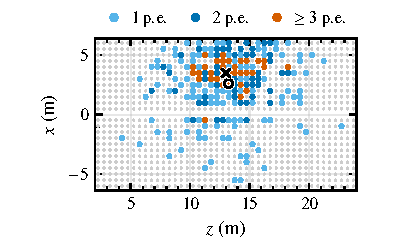
\includegraphics{figures/evento_exemplo.pdf}
    \caption{Long wall at $y = {}$\qty{-6.673}{\m}, the nearest to the vertex, in test event \num{5834} (\qty{387}{\pe} in \num{247} of the \num{6912} channels); it receives most of the light, and all its lit channels are in the part shown. Grey dots: unlit channels; colour: photoelectrons per channel; cross: projection of the vertex; circle: projection of the light centroid, where the global node of the graph sits (Section~\ref{sec:dados_grafos}).}
    \label{fig:evento_exemplo}
  \end{subfigure}\hfill
  \begin{subfigure}[t]{0.485\textwidth}
    \centering
    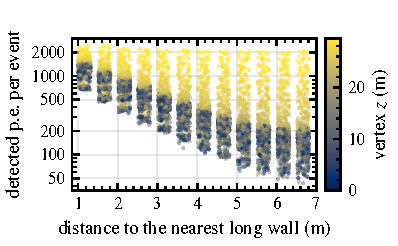
\includegraphics{figures/luz_distancia.pdf}
    \caption{Detected light per event, on a logarithmic scale, for the \num{9364} simulated events, as a function of the distance from the vertex to the nearest long wall; the colour indicates the $z$ coordinate of the vertex. The light falls with distance and is higher near the end cap. The vertices lie at \num{12} distances, \qty{0.5}{\m} apart; the points were shifted at random horizontally to reduce overlap.}
    \label{fig:luz_distancia}
  \end{subfigure}
  \caption{Photon-counting regime: (a) a test event; (b) the light of all simulated events.}
  \label{fig:regime_fotons}
\end{figure}

\subsection{Objective and task formulation}
\label{sec:tarefa}

In the previous stage \citep{vicentin2024study}, a dense network of \num{8195} parameters, fed by \num{60} descriptors selected in phases, obtained a test mean absolute error (MAE) of \num{12.03} to \qty{18.18}{\cm} per axis; since the descriptors summarise the readout of the whole detector, the model receives only what they retain of the light pattern on the channels. This stage represents each event as a graph of the lit channels, estimates the vertex by message passing and compares, on the same test events, \num{11} encoders with almost equal parameter totals (matched capacity), tuned boosters (decision-tree ensembles: XGBoost and LightGBM) and the light barycentre, with the quoted values of the previous network and with APEX at equal detected light. The report also investigates where the error concentrates and what limits it.

The task is to estimate $\mathbf{v}$ from the positions $\mathbf{p}_i$ and the light $n_i$ of the active channels (non-zero $n_i$), which form the set $A$, with $|A|$ elements.

For the predicted vertex $\hat{\mathbf{v}}$ and $J$ events (\num{937} in the test set), the evaluation computes
\begin{equation}
  \begin{aligned}
    \mathrm{MAE}_a &= \bigl\langle \lvert \hat{v}_a - v_a \rvert \bigr\rangle, &\qquad
    \mathrm{RMSE}_a &= \sqrt{\bigl\langle (\hat{v}_a - v_a)^2 \bigr\rangle}, \\
    \mathrm{RMSE}_{\mathrm{comb}} &= \sqrt{\tfrac{1}{3} \textstyle\sum_{a} \mathrm{RMSE}_a^2}, &\qquad
    \bar{d} &= \bigl\langle \lVert \hat{\mathbf{v}} - \mathbf{v} \rVert \bigr\rangle,
  \end{aligned}
  \label{eq:metricas}
\end{equation}
where $\langle\cdot\rangle$ is the mean over the $J$ events, $v_a$ and $\hat{v}_a$ are the components of $\mathbf{v}$ and $\hat{\mathbf{v}}$ along axis $a \in \{x, y, z\}$, $\mathrm{MAE}_a$ and $\mathrm{RMSE}_a$ are the MAE and the root-mean-square error (RMSE) along that axis, $\mathrm{RMSE}_{\mathrm{comb}}$ is the combined RMSE, which does not depend on the assignment of the axes, and $\bar{d}$ is the mean three-dimensional (3-D) error. The mean MAE is the mean of the three $\mathrm{MAE}_a$; $\bar{d}$ is also the training loss and the ranking criterion for the encoders.


\section{Literature Review}

\label{sec:revisao}

\subsection{Position reconstruction from light}
\label{sec:rev_luz}

In noble liquid detectors, the position of a deposit is obtained from the light pattern on the photosensors by light-weighted centroids (biased towards the centre of the array), maximum-likelihood fits to light response functions, or neural networks; in LUX, such a fit reaches a resolution of \qty{0.82}{\cm} in the horizontal position with \num{200} detected photons of electroluminescence (S2) in the gas next to the top array \citep{akerib2018position}. In XENONnT, dense, graph-constrained and convolutional networks estimate this position from the same signal; in simulation, the first two reach about \qty{1.5}{\cm} for an S2 of approximately \qty{100}{\pe} \citep{aprile2025xenonnt}. In DEAP-3600, a single-phase detector, each coordinate comes from a dense network fed by the charges of \num{255} photomultiplier tubes \citep{adhikari2025position}.

In LArTPCs, the light usually provides the trigger and $t_0$ \citep{abratenko2024scintillation, paulucci2022dune}. In an FD2 simulation, the light barycentre has a resolution approximately inversely proportional to the square root of the number of photoelectrons and better than \qty{1}{\m} at low energy \citep{paulucci2022dune}. In SBND, for simulated neutrinos of hundreds of MeV, the position in the plane of the photon detectors comes from the light alone, with a resolution of about \qty{25}{\cm} in the interior and biases of up to \qty{50}{\cm} at the edge \citep{abratenko2024scintillation}. APEX estimates $z$ by the photoelectron-weighted barycentre of the channel coordinates $z_i$, $\bar{z} = \sum_i n_i z_i / \sum_i n_i$; it estimates the horizontal coordinate by the asymmetry between the light of the two long walls and the vertical one by a barycentre corrected by functions of the horizontal one. Its resolution, as a function of energy, is about half that obtained in a similar FD2 simulation \citep{marinho2025apex}.

In JUNO, a liquid scintillator detector, convolutional networks fed by the signals of each photomultiplier tube reconstruct the vertex in simulation to about \qty{10}{\cm} per axis at \qty{1}{\MeV}, four times better than boosted decision trees (Section~\ref{sec:rev_arvores}) and dense networks fed by aggregated features; a graph network was used only for the energy \citep{qian2021vertex}.

\subsection{Graph neural networks}
\label{sec:rev_gnn}

{\displaywidowpenalty=10000 \abovedisplayshortskip=\abovedisplayskip \belowdisplayshortskip=\belowdisplayskip A graph neural network (GNN) operates on a graph $G = (\mathcal{V}, \mathcal{E})$ of nodes $\mathcal{V}$ and directed edges~$\mathcal{E}$. In layer $\ell$, message passing \citep{gilmer2017neural} updates the state~$\mathbf{h}_i^{(\ell)}$ of each node~$i$,
\begin{equation}
  \mathbf{h}_i^{(\ell)} = U^{(\ell)}\Big(\mathbf{h}_i^{(\ell-1)},\ \bigoplus_{j \in \mathcal{N}(i)} M^{(\ell)}\big(\mathbf{h}_i^{(\ell-1)}, \mathbf{h}_j^{(\ell-1)}, \mathbf{e}_{ji}\big)\Big),
  \label{eq:mensagens}
\end{equation}
where $\mathcal{N}(i)$ is the set of incoming neighbours of $i$, the nodes $j$ that have an edge $(j, i)$ with features $\mathbf{e}_{ji}$; $M^{(\ell)}$ and $U^{(\ell)}$ are the message and update functions; and $\oplus$ is a permutation-invariant aggregation. After $L$ layers, each state summarises the neighbourhood within $L$ edges, and a permutation-invariant readout reduces the states to an event vector, used for the regression. The scheme suits a detector, whose active channels vary in number and have no order.\par}

The operators compared differ in the message and in the aggregation: EdgeConv takes the maximum of a network applied to the state and to the difference to each neighbour \citep{wang2019dynamic}; GraphSAGE, the mean \citep{hamilton2017inductive}; GINE, the sum with the edge features \citep{hu2020strategies}; GATv2, a sum weighted by dynamic attention \citep{brody2022how}; ResGatedGCN, a gated sum \citep{bresson2017residual}; GeneralConv, an attention-weighted sum over messages with edge features \citep{you2020design}; PNA combines four aggregators rescaled by the node degree \citep{corso2020principal}; and GPS adds global attention to the local message passing \citep{rampasek2022recipe}. The best design changes from task to task \citep{you2020design}, and comparisons between architectures fix the parameter budget so that the model size does not decide the result \citep{dwivedi2023benchmarking}.

In IceCube, the dynedge network, based on EdgeConv over the pulses of the optical modules, reconstructs the energy, direction and vertex of simulated events between \num{1} and \qty{30}{\GeV} with resolutions on average \num{13} to \qty{20}{\percent} better than those of maximum-likelihood methods \citep{abbasi2022graph}. This work applies the same idea to the scintillation light of \qty{10}{\MeV} deposits in FD3.

\subsection{Gradient-boosted trees}
\label{sec:rev_arvores}

Gradient boosting sums decision trees, each fitted to the residuals of the previous ones; XGBoost and LightGBM, here called boosters, are regularised, fast implementations \citep{chen2016xgboost, ke2017lightgbm}. On medium-sized tabular data, tree ensembles still outperform deep networks \citep{grinsztajn2022why}. Optuna \citep{akiba2019optuna} chooses hyperparameters by Bayesian search with the tree-structured Parzen estimator (TPE) of \citet{bergstra2011algorithms}. The previous stage filtered descriptors by variance, distance correlation, tree-based importance, ablation and Shapley values until the \num{60} inputs of the dense network remained \citep{vicentin2024study}.


% ========== RESULTS OBTAINED ==========
\section{Results}

\label{sec:resultados}

Since the PIBIC report template does not include a methods section, Sections~\ref{sec:dados_grafos} to~\ref{sec:protocolo_comparacao} describe the methods developed in this stage; the results follow in Sections~\ref{sec:codificadores} to~\ref{sec:limites}, the difficulties in Section~\ref{sec:dificuldades} and the changes in Section~\ref{sec:alteracoes}. The encoders were trained and evaluated in the run of 8 August 2026, and the boosters in that of 4 August. For this report, without retraining, the boosters were re-evaluated, and the confidence intervals and the barycentre $\bar{z}$ were computed.

\subsection{Data and graph representation}
\label{sec:dados_grafos}

The vertices in the file names were not in the sensor frame, and the \num{1152} end-cap channels had flipped signs in $y$ and $z$; both corrections were applied during the construction of the dataset and checked on the \num{9364} events. Three hot channels, which had counts in every event and held \qty{47.1}{\percent} of the raw counts, were replaced by the mean of their healthy neighbours: the dataset stores the corrected light. One position was simulated twice, and three files were copies of others. After the corrections, the centroid of the detected light follows the vertex, with a Pearson correlation coefficient $r$ of \num{0.908} in $x$, \num{0.871} in $y$ and \num{0.999} in $z$ over the \num{9364} events.

The events were split into \num{7490} training, \num{937} validation and \num{937} test events, stratified in \num{9} bins per axis (\num{729} groups), a split shared by all models. Given the symmetry of the channels under sign flips of the axes, each training event was mirrored into the other octants: \num{56884} training rows, \num{7.59} per event; the validation and test events stay in the simulated octant. The test vertices lie, on average, \qty{49.31}{\cm} from the nearest training vertex and, except for the position simulated twice, are grid positions absent from the training set: the errors measure interpolation on a \qty{0.5}{\m} grid, with one photon draw per event.

The nodes of the graph $G = (\mathcal{V}, \mathcal{E})$ are the $|A|$ active channels of the event, \num{245} on average in the test events, and one global node \citep{gilmer2017neural} at the light centroid. Each channel receives edges from the $k = {}$\num{4} nearest active channels, in a $k$-nearest-neighbour (\mbox{$k$-NN}) graph, and exchanges one edge in each direction with the global node: six directed edges per channel (\num{248} nodes and \num{1482} edges in the event of Figure~\ref{fig:evento_exemplo}). Each node $i$ has \num{17} features $\mathbf{f}_i$: position, light, light fraction, distance and direction to the centroid, direction to the brightest channel, light of the neighbours, eigenvalues of the light-weighted covariance matrix of the positions (common to all nodes of the event) and light rank. Each edge has \num{23} features $\mathbf{e}_{ji}$: distance, direction, inverse square of the distance, light difference and light similarity, and \num{16} radial basis functions of the distance up to \qty{7}{\m}. The \num{33} event-level scalars, $\mathbf{u}$, are centroids with linear and quadratic weights, total light, number of active channels, largest channel light, spreads, skewnesses and position quantiles. The normalisations use only the training set (\num{8192} sampled graphs), and each vertex coordinate is standardised.

\subsection{Encoders and training protocol}
\label{sec:modelos}

The models (Figure~\ref{fig:arquitetura}) project the \num{17} features $\mathbf{f}_i$ of each node onto an initial state $\mathbf{h}_i^{(0)}$ of width $D$ and apply $L = {}$\num{4} residual layers,
\begin{equation}
  \mathbf{h}_i^{(\ell)} = \mathbf{h}_i^{(\ell-1)} + \mathrm{GELU}\Big(\mathrm{Conv}^{(\ell)}\big(\mathrm{LN}^{(\ell)}(\mathbf{h}_i^{(\ell-1)}),\ \{(\mathrm{LN}^{(\ell)}(\mathbf{h}_j^{(\ell-1)}),\, \mathbf{e}_{ji})\}_{j \in \mathcal{N}(i)}\big)\Big), \quad \ell = 1, \dots, L,
  \label{eq:camada}
\end{equation}
with the layer normalisation $\mathrm{LN}^{(\ell)}$ of \citet{ba2016layer}, the GELU activation (Gaussian error linear unit) of \citet{hendrycks2016gaussian} and the operator $\mathrm{Conv}^{(\ell)}$, which reads $\mathbf{e}_{ji}$ except in EdgeConv, GraphSAGE and ResGatedGCN. In the GPS models, a learned gate mixes a local GATv2, without GELU, with global attention; a residual feed-forward block completes the layer. The readout concatenates the mean, maximum and log-compressed sum of the states. The \num{33} scalars $\mathbf{u}$ enter the regression head both directly and encoded in \num{128} dimensions. The head predicts $x$, then $y$ given the predicted $x$, and $z$ given the predicted $x$ and $y$, also in training, by the feature-wise linear modulation (FiLM) of \citet{perez2018film} or, in the models with the cascade suffix, by concatenation; the suffix designates only the head. A leaky clamp keeps the prediction inside the box \textpm(\num{6.03},~\num{6.67},~\num{29.93})\,\unit{\m}, with a small slope outside it.

\begin{figure}[H]
  \centering
  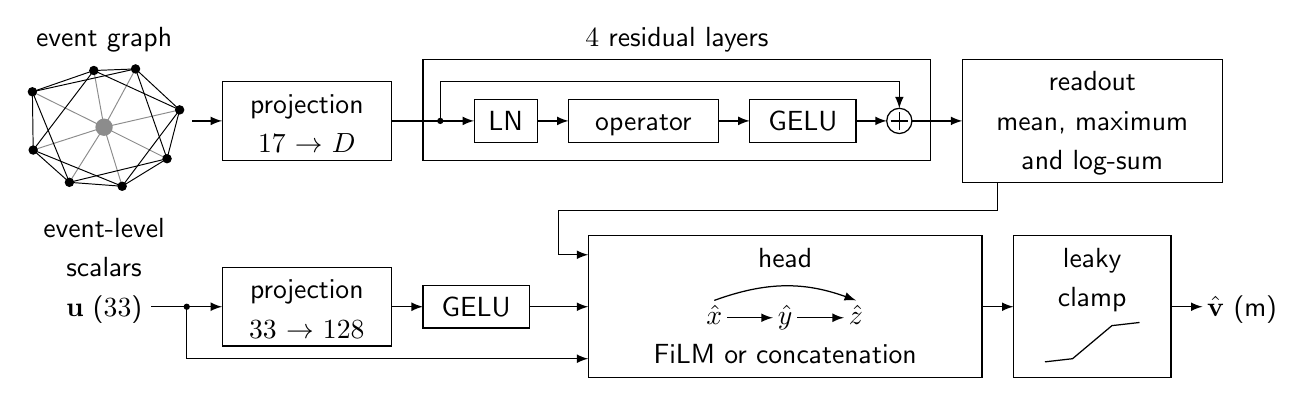
\begin{tikzpicture}[
  x=1cm, y=1cm,
  line width=0.45pt,
  flow/.style={-latex, line width=0.45pt},
  knn/.style={line width=0.35pt},
  spoke/.style={line width=0.35pt, draw=black!45},
  channel/.style={circle, fill=black, inner sep=0pt, minimum size=1.2mm},
  globalnode/.style={circle, fill=black!45, inner sep=0pt, minimum size=2.2mm},
  branch/.style={circle, fill=black, inner sep=0pt, minimum size=0.8mm},
  txt/.style={inner sep=0pt, anchor=base},
  dag/.style={inner sep=1.6pt, execute at begin node={\vphantom{$\hat{x}\hat{y}\hat{z}$}}}
]
\def\arqrowa{3.28}
\def\arqrowb{0.92}
\def\arqgap{2.14}
\def\arqtop{4.22}

\coordinate (g)  at (1.45, 3.20);
\coordinate (c0) at (2.41, 3.42);
\coordinate (c1) at (1.85, 3.94);
\coordinate (c2) at (1.32, 3.92);
\coordinate (c3) at (0.54, 3.65);
\coordinate (c4) at (0.55, 2.91);
\coordinate (c5) at (1.01, 2.50);
\coordinate (c6) at (1.68, 2.45);
\coordinate (c7) at (2.25, 2.80);

\foreach \i in {0,...,7} {\draw[spoke] (g) -- (c\i);}
\foreach \i/\j in {0/1,1/2,2/3,3/4,4/5,5/6,6/7,7/0,0/2,1/3,2/4,3/5,4/6,5/7,6/0,7/1} {\draw[knn] (c\i) -- (c\j);}
\foreach \i in {0,...,7} {\node[channel] at (c\i) {};}
\node[globalnode] at (g) {};
\node[txt] at (1.45, \arqtop) {event graph};

\draw[flow] (2.57, \arqrowa) -- (2.95, \arqrowa);
\draw (2.95, \arqrowa-0.50) rectangle (5.10, \arqrowa+0.50);
\node[txt] at (4.025, \arqrowa+0.10) {projection};
\node[txt] at (4.025, \arqrowa-0.40) {\num{17} $\to$ $D$};

\draw (5.50, \arqrowa-0.50) rectangle (11.95, \arqrowa+0.78);
\node[txt] at (8.725, \arqtop) {\num{4} residual layers};
\draw[flow] (5.10, \arqrowa) -- (6.15, \arqrowa);
\node[branch] at (5.72, \arqrowa) {};
\draw[flow] (5.72, \arqrowa) -- (5.72, \arqrowa+0.50) -- (11.55, \arqrowa+0.50) -- (11.55, \arqrowa+0.16);
\draw (6.15, \arqrowa-0.27) rectangle (6.95, \arqrowa+0.27);
\node[txt] at (6.55, \arqrowa-0.12) {LN};
\draw[flow] (6.95, \arqrowa) -- (7.35, \arqrowa);
\draw (7.35, \arqrowa-0.27) rectangle (9.25, \arqrowa+0.27);
\node[txt] at (8.30, \arqrowa-0.12) {operator};
\draw[flow] (9.25, \arqrowa) -- (9.65, \arqrowa);
\draw (9.65, \arqrowa-0.27) rectangle (11.00, \arqrowa+0.27);
\node[txt] at (10.325, \arqrowa-0.12) {GELU};
\draw[flow] (11.00, \arqrowa) -- (11.39, \arqrowa);
\draw (11.55, \arqrowa) circle (0.16);
\draw (11.44, \arqrowa) -- (11.66, \arqrowa);
\draw (11.55, \arqrowa-0.11) -- (11.55, \arqrowa+0.11);
\draw[flow] (11.71, \arqrowa) -- (12.35, \arqrowa);

\draw (12.35, \arqrowa-0.78) rectangle (15.65, \arqrowa+0.78);
\node[txt] at (14.00, \arqrowa+0.38) {readout};
\node[txt] at (14.00, \arqrowa-0.12) {mean, maximum};
\node[txt] at (14.00, \arqrowa-0.62) {and log-sum};

\draw[flow] (12.80, \arqrowa-0.78) -- (12.80, \arqgap) -- (7.225, \arqgap) -- (7.225, \arqrowb+0.66) -- (7.60, \arqrowb+0.66);

\node[txt] at (1.45, \arqrowb+0.88) {event-level};
\node[txt] at (1.45, \arqrowb+0.38) {scalars};
\node[txt] at (1.45, \arqrowb-0.12) {$\mathbf{u}$ (\num{33})};
\draw[flow] (2.05, \arqrowb) -- (2.95, \arqrowb);
\node[branch] at (2.50, \arqrowb) {};
\draw[flow] (2.50, \arqrowb) -- (2.50, \arqrowb-0.66) -- (7.60, \arqrowb-0.66);
\draw (2.95, \arqrowb-0.50) rectangle (5.10, \arqrowb+0.50);
\node[txt] at (4.025, \arqrowb+0.10) {projection};
\node[txt] at (4.025, \arqrowb-0.40) {\num{33} $\to$ \num{128}};
\draw[flow] (5.10, \arqrowb) -- (5.50, \arqrowb);
\draw (5.50, \arqrowb-0.27) rectangle (6.85, \arqrowb+0.27);
\node[txt] at (6.175, \arqrowb-0.12) {GELU};
\draw[flow] (6.85, \arqrowb) -- (7.60, \arqrowb);

\draw (7.60, \arqrowb-0.90) rectangle (12.60, \arqrowb+0.90);
\node[txt] at (10.10, \arqrowb+0.50) {head};
\node[dag] (xh) at (9.20, \arqrowb-0.14) {$\hat{x}$};
\node[dag] (yh) at (10.10, \arqrowb-0.14) {$\hat{y}$};
\node[dag] (zh) at (11.00, \arqrowb-0.14) {$\hat{z}$};
\draw[flow] (xh) -- (yh);
\draw[flow] (yh) -- (zh);
\draw[flow] (xh.north) to[bend left=20] (zh.north);
\node[txt] at (10.10, \arqrowb-0.72) {FiLM or concatenation};
\draw[flow] (12.60, \arqrowb) -- (13.00, \arqrowb);

\draw (13.00, \arqrowb-0.90) rectangle (15.00, \arqrowb+0.90);
\node[txt] at (14.00, \arqrowb+0.50) {leaky};
\node[txt] at (14.00, \arqrowb) {clamp};
\draw (13.40, \arqrowb-0.70) -- (13.75, \arqrowb-0.66) -- (14.25, \arqrowb-0.24) -- (14.60, \arqrowb-0.20);
\draw[flow] (15.00, \arqrowb) -- (15.40, \arqrowb);
\node[txt, anchor=base west] at (15.45, \arqrowb-0.12) {$\hat{\mathbf{v}}$ (m)};
\end{tikzpicture}\relax

  \caption{Structure shared by the \num{11} encoders. The event graph has one node per active channel and one global node at the light centroid; four residual layers update the node states, which the readout summarises as their mean, maximum and log-compressed sum; the head also receives the \num{33} event-level scalars and predicts $x$, then $y$ given the predicted $x$ ($\hat{x}$), and $z$ given $\hat{x}$ and the predicted $y$ ($\hat{y}$); the leaky clamp keeps the predicted vertex $\hat{\mathbf{v}}$, in metres, inside the box defined by the channels. The encoders differ only in the operator (in the GPS models, the whole layer), the width $D$ and, in the models with the cascade suffix, the head.}
  \label{fig:arquitetura}
\end{figure}

The width $D$ of each encoder was chosen \citep{dwivedi2023benchmarking} so that the parameter total approached that of GPS, \num{1843395}. Of the \num{14} sized encoders, \num{11} were trained (Section~\ref{sec:dificuldades}), with \num{1819019} to \num{1873531} parameters (maximum deviation of \qty{1.6}{\percent}) and $D$ from \num{132} to \num{685}, except for GPS (Table~\ref{tab:codificadores}). The matched capacity is that of the whole model: the encoder's share ranges from \qty{58.3}{\percent} (EdgeConv) to \qty{85.4}{\percent} (GPS-cascade).

The loss $\mathcal{L}$ is the mean Euclidean distance, in metres, between the predicted vertex $\hat{\mathbf{v}}_b$ and the true vertex $\mathbf{v}_b$ of the $B$ rows $b$ of the batch,
\begin{equation}
  \mathcal{L} = \frac{1}{B} \sum_{b=1}^{B} \big\lVert \hat{\mathbf{v}}_b - \mathbf{v}_b \big\rVert,
  \label{eq:perda}
\end{equation}
the same quantity as the mean 3-D error. The AdamW optimiser \citep{loshchilov2019decoupled} used moving-average coefficients of \num{0.9} and \num{0.999}, weight decay of \num{e-4} in the encoder and \num{e-5} in the head, and learning rates of \num{5e-4} and \num{5e-3}, respectively, for batches of \num{128} (\num{1.5e-4} and \num{1.5e-3} in the GPS models), with the rates multiplied by $B$/\num{128} \citep{goyal2017accurate}. The batch size $B$ was the largest power of two, up to \num{512}, that fitted in \qty{20}{\gibi\byte} during a memory probe: \num{128} for four models, \num{256} for two and \num{512} for five. Training used a linear warm-up over \num{100} optimisation steps starting from \num{0.1} times the rate, cosine annealing to \num{e-6} over \num{50} epochs \citep{loshchilov2017sgdr} and gradient-norm clipping at \num{1.0}. The test evaluation used the checkpoint with the lowest validation error; there was no mixed precision, no data augmentation beyond the mirroring and no moving average of the weights. Each encoder was trained once, with seed \num{42}, without a hyperparameter search. The training runs totalled \qty{11.42}{\hour} on a graphics processing unit (GPU) with \qty{23.98}{\gibi\byte} and took \num{5600} to \num{22250} steps: the capacity was matched, but the optimisation budget varied.

\subsection{Reference estimators and uncertainty of the comparisons}
\label{sec:protocolo_comparacao}

On the training rows of the encoders, XGBoost and LightGBM \citep{chen2016xgboost,ke2017lightgbm} fit one regressor per coordinate by least squares to \num{58} aggregated features, such as centroids with linear and quadratic weights, quantiles, spreads, skewnesses and brightest channels. Each regressor has up to \num{3000} trees, and its training stops after \num{100} rounds without improvement on validation; the hyperparameters are those with the lowest mean \mbox{3-D} validation error among \num{40} TPE trials, \num{12} of them random \citep{akiba2019optuna}. In the run records, validation and testing used light with data augmentation (channel dropout and spurious channel activation, noise, gain variation, photon thinning), with \qty{4.1}{\percent} less light in the test set. This report re-evaluates the boosters on the clean light of the encoders; with augmentation, it reproduces the recorded values exactly. The search and the training, however, used augmented light.

The network of the previous stage \citep{vicentin2024study} is quoted rather than re-evaluated: it used a different partition (\qty{80}{\percent} and \qty{20}{\percent}), the geometry prior to the end-cap correction and, judging by its plots, the file-name frame. APEX \citep{marinho2025apex} uses a different simulation (\qty{10}{ppm} of xenon, a field cage reflectivity of \qty{79}{\percent}, light re-emitted by the photon detectors) and analytic estimators. Its resolution widths along its own axes, $\sigma_x$, $\sigma_y$ and $\sigma_z$, read from Figure~2 of the paper at \qty{0.26}{\cm} per pixel, have no published definition; the combined width $\sigma_{\mathrm{comb}}$ is their root mean square. The main comparison is at equal detected light, which does not guarantee equal position information: the mean test light of \qty{530.1}{\pe}\ corresponds to \qty{2.9}{\MeV} in APEX with the average yield, \qty{180}{\pe\per\MeV}, and to \qty{4.9}{\MeV} with the minimum, \qty{109}{\pe\per\MeV}, an energy at which even the dimmest region of APEX gives that much light, which favours APEX; the comparison is also made at equal energy, \qty{10}{\MeV}. Only $\sigma_{\mathrm{comb}}$ and $\sigma_z$ are compared: the correspondence of the transverse widths to $x$ and $y$ is not established.

The barycentre $\bar{z}$, with a quadratic calibration fitted on \num{4000} randomly drawn training events, uses the same \num{937} test events and the same photon draw. The \qty{95}{\percent} intervals come from bootstrap resampling of the test events \citep{efron1979bootstrap}, paired for the encoders and boosters, with \num{10000} shared resamples, and unpaired for the barycentre, with \num{2000}; they cover the sampling of the test set, not the variation between training runs. Because the same test events served the first comparison and the diagnosis that guided the final one (Section~\ref{sec:dificuldades}), the test errors of the encoders may be somewhat optimistic, which the intervals do not cover either. Differences, ratios and percentages are computed without rounding.

\subsection{Comparison of the encoders}
\label{sec:codificadores}

On the test set, the \num{11} encoders lie between \num{25.95} and \qty{28.83}{\cm} in mean 3-D error, a spread of \qty{2.89}{\cm}, with a mean MAE of \num{12.63} to \qty{14.14}{\cm} and a combined RMSE of \num{18.55} to \qty{20.64}{\cm} (Table~\ref{tab:codificadores}). The first four, GATv2-cascade (\qty{25.95}{\cm}), GPS-cascade (\qty{26.06}{\cm}), GATv2 (\qty{26.08}{\cm}) and GPS (\qty{26.27}{\cm}), differ by up to \qty{0.32}{\cm}.

\begin{table}[H]
  \centering
  \caption{The \num{11} encoders of the final comparison, with capacity matched to \num{1843395} parameters, in increasing order of mean 3-D error on the \num{937} test events; mean MAE, combined RMSE and mean 3-D error in cm. $D$: width of the node states; $B$: batch size chosen by the memory probe (\num{128}, \num{256} or \num{512} mirrored training rows, which correspond to \num{22250}, \num{11150} and \num{5600} optimisation steps over \num{50} epochs, respectively), with the learning rates multiplied by $B$/\num{128}. $^{\dagger}$: does not read the edge features. The first four cannot be distinguished by the paired resampling (Figure~\ref{fig:diferenca_pareada}).}
  \label{tab:codificadores}
  \begin{tabular}{@{}l S[table-format=3.0] S[table-format=1.3] S[table-format=3.0] S[table-format=2.2] S[table-format=2.2] S[table-format=2.2]@{}}
\toprule
 & {} & {Parameters} & {} & {Mean} & {RMSE} & {Mean 3-D} \\
Encoder & {$D$} & {(\num{e6})} & {$B$} & {MAE (cm)} & {comb.\ (cm)} & {error (cm)} \\
\midrule
GATv2-cascade & 212 & 1.869 & 128 & 12.63 & 18.64 & 25.95 \\
GPS-cascade & 132 & 1.874 & 128 & 12.79 & 18.69 & 26.06 \\
GATv2 & 204 & 1.819 & 128 & 12.74 & 18.80 & 26.08 \\
GPS & 128 & 1.843 & 256 & 12.95 & 18.55 & 26.27 \\
GeneralConv & 280 & 1.833 & 256 & 12.86 & 18.94 & 26.43 \\
ResGatedGCN$^{\dagger}$ & 292 & 1.841 & 512 & 13.07 & 19.02 & 26.71 \\
GraphSAGE$^{\dagger}$ & 400 & 1.840 & 512 & 13.23 & 19.01 & 26.92 \\
EdgeConv$^{\dagger}$ & 685 & 1.843 & 128 & 13.46 & 20.23 & 27.67 \\
PNA & 147 & 1.841 & 512 & 13.52 & 19.57 & 27.68 \\
GINE & 395 & 1.844 & 512 & 13.81 & 20.21 & 28.23 \\
GINE-cascade & 404 & 1.843 & 512 & 14.14 & 20.64 & 28.83 \\
\bottomrule
\end{tabular}

\end{table}

The paired differences in mean 3-D error relative to GATv2-cascade are \qty[retain-explicit-plus]{+0.12}{\cm} (\num{-0.30} to \qty{0.54}{\cm}) for GPS-cascade, \qty[retain-explicit-plus]{+0.13}{\cm} (\num{-0.28} to \qty{0.55}{\cm}) for GATv2 and \qty[retain-explicit-plus]{+0.32}{\cm} (\num{-0.12} to \qty{0.77}{\cm}) for GPS, intervals that contain zero; from GeneralConv onwards (\qty[retain-explicit-plus]{+0.48}{\cm}; \num{0.02} to \qty{0.95}{\cm}), the intervals lie above zero, without correction for multiple comparisons (Figure~\ref{fig:diferenca_pareada}). GATv2-cascade has the lowest mean 3-D error in \qty{56.9}{\percent} of the resamples; GPS, with the lowest combined RMSE (\qty{18.55}{\cm}), leads that metric in \qty{61.8}{\percent} of them; GATv2 has the lowest validation error (\qty{25.72}{\cm}). There is, therefore, no established best encoder. From here on, GATv2-cascade represents the group of the four best; it was chosen by the test metric, a choice that favours its test error, and was trained once, like the others.

Early stopping (\num{15} epochs without improvement on validation) was not triggered; the lowest validation error occurred between epochs \num{41} and \num{50}, in the last epoch for GraphSAGE and GeneralConv. For GATv2-cascade (Figure~\ref{fig:curvas_validacao}), the training error on the mirrored rows ends at \qty{21.91}{\cm}, and the validation and test errors agree (\num{25.96} and \qty{25.95}{\cm}).

\begin{figure}[H]
  \centering
  \begin{subfigure}[t]{0.485\textwidth}
    \centering
    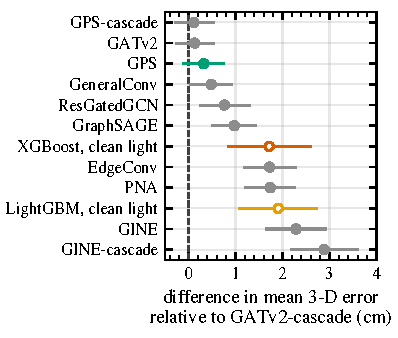
\includegraphics{figures/diferenca_pareada.pdf}
    \caption{Difference in mean 3-D test error relative to that of GATv2-cascade, with a \qty{95}{\percent} interval from paired bootstrap resampling of the \num{937} test events (\num{10000} resamples); GPS, with the lowest combined RMSE, in green; \mbox{XGBoost} and \mbox{LightGBM} on clean light, with hollow markers. Positive differences indicate a higher error than that of GATv2-cascade; the intervals of GPS-cascade, GATv2 and GPS contain zero.}
    \label{fig:diferenca_pareada}
  \end{subfigure}\hfill
  \begin{subfigure}[t]{0.485\textwidth}
    \centering
    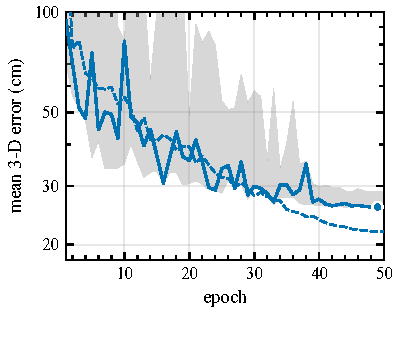
\includegraphics{figures/curvas_validacao.pdf}
    \caption{Mean 3-D error per epoch, on a logarithmic scale: shaded band between the lowest and the highest validation error of the \num{11} encoders and, for GATv2-cascade, the validation curve (solid) and the training curve on the mirrored rows (dashed), with a marker at the epoch of lowest validation error. The training value of the first epoch and the upper edge of the band at several epochs of the first half of training lie above the scale.}
    \label{fig:curvas_validacao}
  \end{subfigure}
  \caption{Comparison of the \num{11} matched-capacity encoders: (a) differences on the \num{937} test events; (b) training curves.}
  \label{fig:par_codificadores}
\end{figure}

The three encoders that do not read the edge features sit in the middle of Table~\ref{tab:codificadores}: ResGatedGCN sixth, GraphSAGE seventh and EdgeConv eighth. The five trained with batch size \num{512} (\num{5600} steps) occupy positions 6, 7, 9, 10 and 11, and the first three used batch size \num{128} (\num{22250} steps): the comparison equalises the number of parameters but does not separate the effect of the operator from that of the optimisation budget.

\subsection{Comparison with the reference estimators}
\label{sec:comparacao_referencias}

On clean light, GATv2-cascade has a mean 3-D error \qty{1.71}{\cm} lower than that of XGBoost (\num{0.83} to \qty{2.62}{\cm}) and a combined RMSE \qty{2.30}{\cm} lower (\num{1.66} to \qty{2.95}{\cm}); against LightGBM, \num{1.91} and \qty{1.98}{\cm} (Figure~\ref{fig:diferenca_pareada} and Table~\ref{tab:referencias}). By the point estimates, seven of the \num{11} encoders have a mean 3-D error lower than that of XGBoost, but GATv2-cascade lands closer to the vertex than XGBoost in only \qty{47.6}{\percent} of the events: XGBoost errs less on the brightest events, and GATv2-cascade on the dimmest ones and in the tail, with the 90th percentile of the \mbox{3-D} error at \qty{51.26}{\cm} against \qty{60.26}{\cm} (Section~\ref{sec:onde_erro}). In the run records, on augmented light, XGBoost has a mean MAE of \qty{13.01}{\cm} and a combined RMSE of \qty{20.82}{\cm}, against \num{13.21} and \qty{20.95}{\cm} on clean light.

Compared with the network of the previous stage \citep{vicentin2024study}, with values obtained on a different partition and in the geometry prior to the corrections, the combined RMSE of GATv2-cascade is \qty{10.6}{\percent} lower (\num{18.64} against \qty{20.86}{\cm}) and its mean MAE \qty{16.5}{\percent} lower (\num{12.63} against \qty{15.13}{\cm}). Per axis, in the sensor frame, the RMSE falls by \num{4.23} and \qty{1.81}{\cm} in $x$ and $y$, and in $z$ the value of that network, \qty{0.41}{\cm} higher, lies within the \qty{95}{\percent} interval of GATv2-cascade. On clean light, the boosters lie within \qty{0.24}{\cm} of the combined RMSE of that network, and the \num{11} encoders lie below it, between \num{18.55} and \qty{20.64}{\cm}; for EdgeConv, GINE and GINE-cascade, as for the boosters, the value of that network lies within the \qty{95}{\percent} interval.

\begin{table}[H]
  \centering
  \caption{Test errors of GATv2-cascade, GPS and the reference estimators, in cm, in the sensor frame; the barycentre has a quadratic calibration. \textsuperscript{a}Quoted per-axis RMSE values, from a different partition (\qty{80}{\percent} and \qty{20}{\percent}) and from the geometry prior to the corrections \citep{vicentin2024study}, with the axes converted to this frame; combined RMSE and mean MAE computed from the published per-axis values. \textsuperscript{\smash{b}}A different simulation \citep{marinho2025apex}; widths read from Figure~2 of the paper at \qty{0.26}{\cm} per pixel, at equal detected light with the average yield (\qty{2.9}{\MeV}) or with the minimum (\qty{4.9}{\MeV}) and at equal energy (\qty{10}{\MeV}); the two transverse widths appear in the same cell, without assignment to $x$ and $y$; MAE not available.}
  \label{tab:referencias}
  \begin{tabular}{@{}l S[table-format=2.2] S[table-format=2.2] S[table-format=2.2] S[table-format=2.2] S[table-format=2.2]@{}}
\toprule
 & {RMSE $x$} & {RMSE $y$} & {RMSE $z$} & {RMSE} & {Mean} \\
Estimator & {(cm)} & {(cm)} & {(cm)} & {comb.\ (cm)} & {MAE (cm)} \\
\midrule
GATv2-cascade & 20.45 & 14.35 & 20.46 & 18.64 & 12.63 \\
GPS & 20.55 & 14.29 & 20.15 & 18.55 & 12.95 \\
\midrule
XGBoost, clean light & 23.82 & 16.96 & 21.47 & 20.95 & 13.21 \\
LightGBM, clean light & 23.91 & 16.55 & 20.75 & 20.62 & 13.38 \\
Barycentre ($z$ only) &  &  & 42.45 &  &  \\
\midrule
Dense network (2024)\textsuperscript{a} & 24.68 & 16.16 & 20.87 & 20.86 & 15.13 \\
APEX, \qty{2.9}{\MeV}\textsuperscript{b} & \multicolumn{2}{c}{\num{33.1} and \num{51.3}} & 24.8 & 38.0 &  \\
APEX, \qty{4.9}{\MeV}\textsuperscript{b} & \multicolumn{2}{c}{\num{26.8} and \num{44.0}} & 19.4 & 31.8 &  \\
APEX, \qty{10}{\MeV}\textsuperscript{b} & \multicolumn{2}{c}{\num{20.8} and \num{37.3}} & 13.7 & 25.9 &  \\
\bottomrule
\end{tabular}

\end{table}

At detected light equal to the test mean and with the average yield, the combined width of APEX \citep{marinho2025apex} is \qty{38.0}{\cm}, and the combined RMSE of GATv2-cascade, \qty{18.64}{\cm} (\num{17.69} to \qty{19.61}{\cm}), is \qty{51.0}{\percent} lower; with the minimum yield, it is \qty{41.3}{\percent} lower than the width of \qty{31.8}{\cm}, and at equal energy, \qty{28.0}{\percent} lower than that of \qty{25.9}{\cm} (Figure~\ref{fig:apex_luz}). In $z$, against \num{20.15} to \qty{20.46}{\cm} for the four best, APEX has \qty{24.8}{\cm} with the average yield, above the \qty{95}{\percent} interval of each of them, and \qty{19.4}{\cm} with the minimum, within it; only at equal energy (\qty{13.7}{\cm}) is it better. The paper does not define the width: at \qty{4}{\MeV}, the plotted value is \num{0.96} times the standard deviation and \num{1.13} times the Gaussian width of the residuals in $z$; a Gaussian width, smaller than the standard deviation, would favour APEX against an RMSE.

{\clubpenalty=10000 On the same events, the barycentre $\bar{z}$ \citep{marinho2025apex}, here with a quadratic calibration, has an RMSE in $z$ of \qty{42.45}{\cm} (\num{39.55} to \qty{45.22}{\cm}; \qty[uncertainty-mode = separate, separate-uncertainty-units = single]{41.98 \pm 0.61}{\cm}, mean and standard deviation over \num{30} photon draws; Figure~\ref{fig:baricentro_luz}), \num{2.07} times that of GATv2-cascade, and with a cubic calibration, \qty{41.86}{\cm}. Without calibration, the barycentre has \qty{66.59}{\cm}, shifted on average by \qty{34.08}{\cm} towards the nearest end cap, mainly for the vertices from $z = {}$\qty{20}{\m} upwards (Section~\ref{sec:onde_erro}), a bias not found in APEX. Of the single-statistic estimators tested, the barycentre of all channels is the best (with a cubic calibration, barycentre of only the channels more than \qty{1}{\m} from the end caps: \qty{66.95}{\cm}; brightest channel: \qty{142.16}{\cm}).\par}

\begin{figure}[H]
  \centering
  \begin{subfigure}[t]{0.485\textwidth}
    \centering
    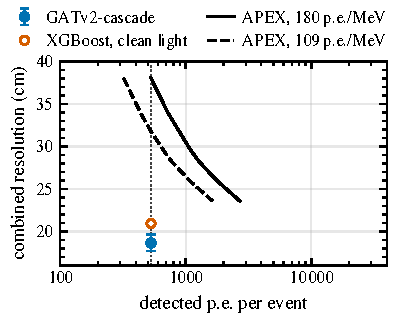
\includegraphics{figures/apex_luz.pdf}
    \caption{Combined width of APEX in a different simulation \citep{marinho2025apex}, with the energy converted into photoelectrons by the average yield (\qty{180}{\pe\per\MeV}; \qty{10}{\MeV} gives \qty{1800}{\pe}) and by the minimum (\qty{109}{\pe\per\MeV}), and the combined RMSE of GATv2-cascade (\qty{95}{\percent} interval) and of \mbox{XGBoost} on clean light, at the mean test light (\qty{530.1}{\pe}, dotted line).}
    \label{fig:apex_luz}
  \end{subfigure}\hfill
  \begin{subfigure}[t]{0.485\textwidth}
    \centering
    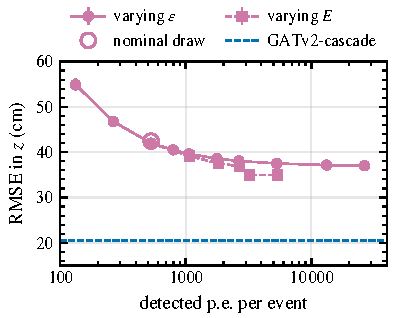
\includegraphics{figures/baricentro_luz.pdf}
    \caption{RMSE in $z$ of the barycentre with a quadratic calibration, on the test set, varying the efficiency $\varepsilon$ from \num{0.005} to \num{1}, with $E$ fixed at \qty{10}{\MeV}, or the energy $E$ from \num{10} to \qty{100}{\MeV}, with $\varepsilon$ fixed at \num{0.02}: mean over \num{30} photon draws and standard deviation (bars, smaller than the markers except at $\varepsilon = {}$\num{0.005}); hollow circle: nominal draw, used for training and testing the models; horizontal line: GATv2-cascade, evaluated on that draw only.}
    \label{fig:baricentro_luz}
  \end{subfigure}
  \caption{Resolution as a function of the detected light per event, for the analytic estimators and, at the test light only, for the models: (a) combined over the three axes; (b) in $z$.}
  \label{fig:par_luz_referencias}
\end{figure}

\subsection{Where the error concentrates}
\label{sec:onde_erro}

The per-event 3-D error falls with the detected light: the Spearman rank correlation $\rho_{\mathrm{S}}$ is \num{-0.68} for GATv2-cascade and \num{-0.72} for XGBoost on clean light. By test-light quartile (boundaries: \num{201}, \num{387} and \qty{773}{\pe}), the mean 3-D error of GATv2-cascade is \num{42.79}, \num{31.25}, \num{18.19} and \qty{11.67}{\cm}, and that of XGBoost is \num{47.28}, \num{35.74}, \num{20.78} and \qty{6.98}{\cm} (Figure~\ref{fig:erro_luz}): GATv2-cascade errs less in the three dimmest quartiles (paired differences with intervals above zero), and XGBoost errs less in the brightest, by \qty{4.70}{\cm} (\num{3.58} to \qty{5.75}{\cm}). The centroids with quadratic and linear weights account for \num{43.5} and \qty{33.3}{\percent}, respectively, of the gain importance of XGBoost, trained on augmented light. Since both become more precise with more light, this is consistent with the advantage of XGBoost in the bright events but does not explain it: GATv2-cascade receives the same two centroids among the event-level scalars (Section~\ref{sec:dados_grafos}), and the cause of its larger error in these events was not investigated.

In the sensor frame, the $y$ axis, normal to the long walls, has the lowest RMSE for GATv2-cascade (\qty{14.35}{\cm}, against \num{20.45} and \qty{20.46}{\cm} in $x$ and $z$), for GPS, for the boosters on clean light and for the network of the previous stage (axes converted by an inferred correspondence; Table~\ref{tab:referencias}). The $x$ axis, normal to the faces without channels, has the highest for the boosters (XGBoost: \qty{23.82}{\cm}) and for that network (\qty{24.68}{\cm}). The coefficient of determination $R^2$ of GATv2-cascade in $z$, the fraction of the variance explained, is \num{0.9994} because the standard deviation of the test vertices is \num{4.6} times as large in $z$ as in $x$, not because $z$ is better reconstructed.

Below $z = {}$\qty{20}{\m} (\num{626} events), the RMSE values in $z$ of the calibrated barycentre, of GATv2-cascade and of XGBoost on clean light are close to one another (\num{23.29}, \num{22.54} and \qty{22.63}{\cm}); from \qty{20}{\m} upwards (\num{311} events), that of the barycentre rises to \qty{65.87}{\cm}, and the other two fall to \num{15.44} and \qty{18.91}{\cm} (Figure~\ref{fig:erro_z}). The factor \num{2.07} of Section~\ref{sec:comparacao_referencias} comes from these vertices: the channels of the end cap, all at $z = {}$\qty{29.93}{\m}, receive \qty{41.2}{\percent} of the light and shift the barycentre all the more the further the vertex lies from the long walls, which the calibration, a function of $\bar{z}$ alone, does not correct.

\begin{figure}[H]
  \centering
  \begin{subfigure}[t]{0.485\textwidth}
    \centering
    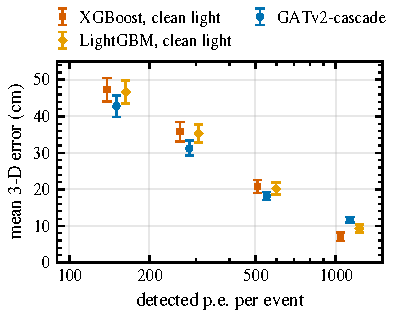
\includegraphics{figures/erro_luz.pdf}
    \caption{Mean 3-D error of GATv2-cascade and, on clean light, of \mbox{XGBoost} and \mbox{LightGBM}, by quartile of the detected light in the \num{937} test events; points at the mean light of the quartile, those of the boosters offset sideways, and \qty{95}{\percent} bars on each mean, from a bootstrap over the events of the quartile. GATv2-cascade errs less in the three dimmest quartiles, and \mbox{XGBoost} in the brightest (\qty{773}{\pe} or more); the interval of the paired difference between the two excludes zero in every quartile.}
    \label{fig:erro_luz}
  \end{subfigure}\hfill
  \begin{subfigure}[t]{0.485\textwidth}
    \centering
    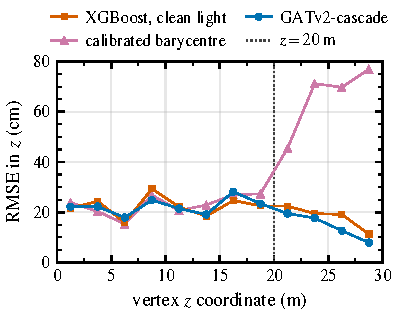
\includegraphics{figures/erro_z.pdf}
    \caption{RMSE in $z$ of GATv2-cascade, of the calibrated barycentre and of \mbox{XGBoost} on clean light in the test events, per \qty{2.5}{\m} bin of the vertex $z$; dotted line at \qty{20}{\m}. Up to \qty{20}{\m}, the errors are close to one another; near the end cap ($z = {}$\qty{29.93}{\m}), that of the barycentre rises and that of GATv2-cascade falls.}
    \label{fig:erro_z}
  \end{subfigure}
  \caption{Where the error concentrates in the test events: (a)~by quartile of detected light; (b)~by bin of the vertex $z$.}
  \label{fig:par_onde_erro}
\end{figure}

\subsection{What limits the resolution}
\label{sec:limites}

In the nominal draw of the test set, the RMSE in $z$ of the calibrated barycentre falls from \num{55.18} to \qty{37.02}{\cm} between efficiencies $\varepsilon$ of \num{0.005} and \num{1}, and from \num{42.45} to \qty{35.24}{\cm} between energies of \num{10} and \qty{100}{\MeV} (Figure~\ref{fig:baricentro_luz} shows means). With \qty{177.8}{\pe\per\MeV} on average, near the average yield of APEX, it stands at \qty{38.23}{\cm} and, below $z = {}$\qty{20}{\m}, with less light, at \qty{13.79}{\cm}, close to the \qty{13.7}{\cm} obtained by APEX at \qty{10}{\MeV} (Table~\ref{tab:referencias}). Detecting every photon would reduce the error of the barycentre by \qty{5.43}{\cm} (\qty{4.96}{\cm} averaged over the draws), and by more still without the rounding of Equation~\eqref{eq:luz}, which at \qty{10}{\MeV} sets the weakest channels to zero and raises this error; for this reason, at the same detected light, the energy sweep lies below the efficiency sweep. Over the whole test set, the error of the barycentre is mainly systematic: with $\varepsilon = {}$\num{0.02}, GATv2-cascade (\qty{20.46}{\cm}) already errs less in $z$ than the barycentre with every photon. This systematic part is due to the vertices from \qty{20}{\m} upwards, where the barycentre stays at \qty{63.16}{\cm} even with every photon (Section~\ref{sec:onde_erro}); below \qty{20}{\m}, its error is mainly statistical: from \qty{23.29}{\cm}, near GATv2-cascade (\qty{22.54}{\cm}), it falls to \qty{8.33}{\cm} with every photon.

The error of GATv2-cascade also falls with more light (Section~\ref{sec:onde_erro}), but the light decreases away from the long walls, and the models were trained only at \qty{10}{\MeV} and $\varepsilon = {}$\num{0.02}: for them, no sweep separates the effect of photon statistics from that of position. The influence of the grid coverage was not isolated. With the full training set, every test vertex has a training vertex at most \qty{50}{\cm} away; with a quarter of the events, as in the first comparison (Section~\ref{sec:dificuldades}), \qty{27.6}{\percent} of the test vertices lack such a neighbour, and the mean distance rises from \num{49.31} to \qty{56.18}{\cm}. The models also read \num{33} hand-crafted event-level scalars, and, in the final configuration, no experiment separated the contribution of message passing from that of the scalars: the result is that of the graph encoders with these scalars, not of message passing or of the graph representation alone.

\subsection{Difficulties Encountered}
\label{sec:dificuldades}

The data had two geometry defects, one hidden by the other: vertices and channels in different frames; end caps rotated about $x$, with $y$ and $z$ inverted. Both were identified from the light pattern, and the existing models were retrained. Format changes without backward compatibility made the old checkpoints unusable, and no run from before 4 August 2026 remains.

In the first comparison, on 4 August 2026, the encoders used a quarter of the training events (\num{1872}), without mirroring, and \num{9} event-level scalars; the lowest mean test MAE was \qty{18.05}{\cm}, against \qty{13.01}{\cm} for XGBoost, both on augmented light. A diagnosis recorded during the project, not reproduced in this report, attributed about \qty{1.9}{\cm} of the gap to the size of the training set, \qty{1.9}{\cm} to the missing aggregated features, \qty{1.0}{\cm} to the hyperparameter search and the mirroring of the boosters, and \qty{0.3}{\cm} to the remainder, the joint contribution of nodes, edges and message passing. Measured on the test events of the final comparison, it led to the adoption of the full training set, the \num{33} scalars and the evaluation right after each training run. The final comparison changed these and other settings at once and used clean light; in it, the lowest mean MAE was \qty{12.63}{\cm}.

The local GPU had \qty{3.63}{\gibi\byte}: in the models with global attention, graphs with all \num{6912} channels fitted only in very small batches, hence the restriction to the active channels; in the first comparison, GCN, TransformerConv and GPS-lite failed for lack of memory. The final comparison, on another GPU with \qty{23.98}{\gibi\byte}, stopped without an error message after training \num{11} of the \num{14} encoders; the same three were missing.

The boosters were evaluated on light with data augmentation, with a mean test light \qty{4.1}{\percent} lower than that of clean light; re-evaluated on clean light in this report, XGBoost has a mean MAE \qty{0.20}{\cm} higher (Sections~\ref{sec:protocolo_comparacao} and~\ref{sec:comparacao_referencias}).

\subsection{Changes to the Project}
\label{sec:alteracoes}

With respect to the initial plan, the representation changed from \num{60} descriptors with a dense network to graphs of the active channels, because the descriptors summarise the readout of the whole detector; the final models, however, still read \num{33} hand-crafted event-level scalars. Instead of a single architecture, the project compared \num{11} matched-capacity encoders, so that the number of parameters would not decide the result. Boosters fitted to aggregated features were added as reference models after a simple gradient-boosting model outperformed the GNN of the time in July 2026. The evaluation changed from a partition of \qty{80}{\percent} and \qty{20}{\percent}, with \num{10}-fold cross-validation, to a fixed stratified split of \num{7490}, \num{937} and \num{937} events, shared by all models; the final comparison had no cross-validation. APEX was compared at equal energy and also at equal detected light, because its simulation has an average light yield of \qty{180}{\pe\per\MeV}, \num{3.4} times that of the test set, \num{53.0}.

The extension to other energies and geometries, envisaged in the plan, was not carried out with the final models; what remained was the efficiency and energy sweep of the barycentre (Section~\ref{sec:limites}). The final comparison trained the encoders without the hyperparameter search of the plan (Section~\ref{sec:modelos}), which was applied only to the boosters (Section~\ref{sec:protocolo_comparacao}). Of the planned per-axis metrics, the report retains the RMSE, the mean of the three MAE values and $R^2$, the last in $z$ only (Section~\ref{sec:onde_erro}); the ranking and the training loss use the mean 3-D error (Section~\ref{sec:tarefa}). The comparison with APEX, proposed per coordinate, was restricted to $z$ and the combined width, because the correspondence of the transverse widths to $x$ and $y$ is not established (Section~\ref{sec:protocolo_comparacao}). Use in real-time data acquisition, expected in the plan, was not evaluated: the inference time was not measured, and the encoders, with capacity matched to \num{1843395} parameters, are larger than the network of the previous stage, with \num{8195}. That network is quoted rather than re-evaluated, because it used a different partition and the geometry prior to the corrections and because the trained model is not available.



% ========== CONCLUSIONS ==========
\section{Conclusions}

\label{sec:conclusoes}

The message-passing encoders on the graph of the active channels, with the event-level scalars, reconstruct the vertex of \qty{10}{\MeV} deposits (a mean of \qty{530.1}{\pe} per test event) with a mean 3-D error of \num{25.95} to \qty{26.27}{\cm} and a combined RMSE of \num{18.55} to \qty{18.80}{\cm} for the four best. At matched capacity, the mean 3-D error of the \num{11} encoders varies by up to \qty{2.89}{\cm}, and these four cannot be distinguished on the \num{937} test events. GATv2-cascade, chosen for the lowest mean 3-D test error, has a per-axis RMSE, in the sensor frame, of \num{20.45}, \num{14.35} and \qty{20.46}{\cm} in $x$, $y$ and $z$.

On the same events and on clean light, GATv2-cascade has a mean 3-D error \qty{1.71}{\cm} lower than that of XGBoost and a combined RMSE \qty{2.30}{\cm} lower; it is better on the dim events and in the tail, but worse in the brightest quartile. In $z$, the calibrated barycentre has an RMSE \num{2.07} times that of GATv2-cascade because of the vertices near the end cap, where the error of the barycentre is systematic, a bias that APEX did not find in its simulation. Below $z = {}$\qty{20}{\m}, the barycentre stays close to GATv2-cascade (\num{23.29} and \qty{22.54}{\cm}), and its error is mainly statistical: with every photon detected, it falls to \qty{8.33}{\cm}. The combined RMSE of GATv2-cascade is \qty{10.6}{\percent} lower than that of the network of the previous stage, a value computed from the published per-axis values, which come from a different partition and from the geometry prior to the corrections; the difference is in $x$ and $y$, since in $z$ the value of that network, \qty{20.87}{\cm}, lies within the \qty{95}{\percent} interval of GATv2-cascade. At equal detected light with the average yield, this combined RMSE is \qty{51.0}{\percent} lower than the combined width of APEX (\qty{41.3}{\percent} with the minimum and \qty{28.0}{\percent} at equal energy), a root mean square of widths with no published definition, read from a plot of a different simulation. In~$z$, against \qty{20.46}{\cm} for GATv2-cascade, APEX has \qty{24.8}{\cm} with the average yield, above the \qty{95}{\percent} interval, and \qty{19.4}{\cm} with the minimum, within it; only at equal energy, where it detects \num{3.4} times as much light, is it better (\qty{13.7}{\cm}).

{\clubpenalty=10000 The error of GATv2-cascade concentrates in the dim events, far from the long walls (a~mean 3-D error of \qty{42.79}{\cm} in the dimmest quartile, against \qty{11.67}{\cm} in the brightest), but the effect of photon statistics was not separated from that of position. The results hold for one energy, one efficiency, one geometry, one photon draw per event and vertices on the training grid. Each encoder was trained once, without the hyperparameter search carried out for the boosters, with different batch sizes and numbers of steps; there was no ablation of the \num{33} scalars; the boosters were trained on augmented light; and the test events had already guided the final design of the encoders.\par}

{\clubpenalty=10000 As future work, this report proposes training and evaluating the encoders for several efficiencies, energies and geometries; generating several photon draws per event and vertices off the grid; repeating the comparison with a fixed optimisation budget, a hyperparameter search per encoder, boosters tuned and trained on clean light, and several seeds, with and without the scalars, on new test events; predicting the coordinates from the channel states, so as to test whether summarising the graph in a single vector limits the precision; combining boosters and encoders, which err less in different light ranges; comparing with APEX in an equivalent simulation, confirming the correspondence of the axes and the definition of the width; and measuring the inference time per event.\par}


% ========== ACKNOWLEDGEMENTS ==========
\phantomsection
\section*{Acknowledgements}
\addcontentsline{toc}{section}{Acknowledgements}

\label{sec:agradecimentos}

The author thanks CNPq for the undergraduate research scholarship granted through the PIBIC-ITA Programme.

The author thanks the supervisor, \nomeorientador, for the guidance and support during the development of this research.


% ========== BIBLIOGRAPHY ==========
\newpage
\phantomsection
\addcontentsline{toc}{section}{\refname}
\bibliographystyle{abbrvnat}
\bibliography{referencias}

\end{document}
